\documentclass[a4paper,twoside]{article}
\usepackage[T1]{fontenc}
%\usepackage[encapsulated]{CJK}
\usepackage[utf8]{inputenc}
\usepackage{mathptmx}
\usepackage[scaled=0.9]{helvet}
\usepackage{courier}
\usepackage{pifont}
\usepackage{pdfpages}
\usepackage{fancyhdr}
%\usepackage{hyperref}
\usepackage{qrcode}
\usepackage[%
%  keepfiles,
  reusefiles
]{abcsvgintex}
\abcsvgauxdir{./abcsvgtmp/}
%\usepackage{ean13isbn}

\usepackage[top=2cm,bottom=2cm,left=1.5cm,right=1.5cm]{geometry}

\newcommand{\anneecopyright}{2014-2025}

%\renewcommand{\ocrb}{%
%%  \usefont{T1}{pcr}{m}{n}\fontsize{11pt}{11pt}\selectfont%
%%  \usefont{T1}{pcr}{b}{n}\fontsize{11pt}{11pt}\selectfont%
%  \usefont{T1}{phv}{m}{n}\fontsize{13pt}{11pt}\selectfont\X=1pt
%}
%\def\EANfinal{\testconsistence
%  \kern7\X\egroup
%  \hbox{\ocrbsmall \kern10\X \ISBNnum}\kern1\X
%  \dp0=0pt \box0 \kern1\X
%  \hbox{\ocrb\kern2\X\firstdigit\kern5\X \frontdigits\kern5\X \enddigits}
%  \egroup \global\barheight=0pt \gdef\ISBNnum{}}

\setlength{\parindent}{0pt}

\newcommand{\includerh}[3][0pt]{%
  \raisebox{#1}{\includegraphics[height=#2]{#3}}%
}
\makeatletter
\newcommand{\isodate}{%
  \the\year-\ifnum\the\month<10 0\fi\the\month-\ifnum\the\day<10 0\fi\the\day~
  \@tempcnta=\time
  \@tempcntb=\@tempcnta
  \divide\@tempcntb by 60
  \multiply\@tempcntb by 60
  \advance\@tempcnta by -\@tempcntb
  \divide\@tempcntb by 60
  \the\@tempcntb :\ifnum\the\@tempcnta < 10 0\fi\the\@tempcnta
}
\makeatother
\begin{document}
\pagestyle{empty}
\begin{titlepage}
  \newgeometry{nohead,nofoot,top=0.5cm,bottom=1cm,left=1cm,right=1cm}%
  \vspace*{\fill}%
  \hspace*{\fill}\fbox{\parbox[c][0.95\textheight][c]{0.95\textwidth}{%
    \vspace*{0pt plus 0.7 fill}
    \begin{center}
      \LARGE
      Jean-Sébastien Bach
      
      \bigskip
      
      \Huge
      Suites pour violoncelle
      
      \bigskip
      
      \Large
      BWV 1007-1012
      

    \vspace*{0pt plus 0.3 fill}

%    \includegraphics{inc/BasseUtBuffet}
    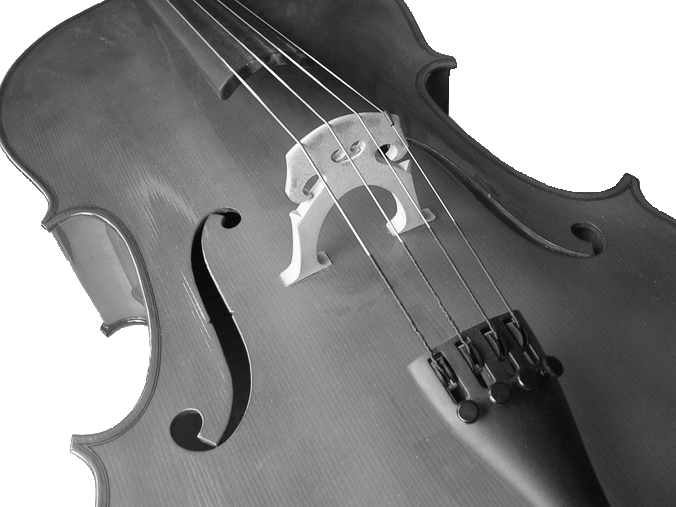
\includegraphics[scale=0.5]{inc/CelloCloseup1_gray}
    
    \vspace*{0pt plus 0.5 fill}

    \normalsize\sffamily
    
    \copyright oclaribou editions \anneecopyright\quad frederic@oclaribou.fr
    
    https://www.oclaribou.fr/MusicBJS/BJSCelloSuites
        
    \bigskip
    
    \small
    http://creativecommons.org/licenses/by-sa/3.0/
    
    \smallskip
    
    
\includegraphics[width=2cm]{inc/by-sa}

    \end{center}
    \vspace*{0pt plus 0.1 fill}
  }}\hspace*{\fill}
  \vspace*{\fill}
\end{titlepage}
\restoregeometry

\cleardoublepage
%% page impaire
  \newgeometry{nohead,nofoot,top=0.5cm,bottom=1cm,left=1cm,right=1cm}%
  \vspace*{\fill}
  \begin{center}
	\LARGE
	Jean-Sébastien Bach
	
	\bigskip
	
	\Huge
	Suites pour violoncelle
	
	\bigskip
	
	\Large
	BWV 1007-1012
	
	
	\vspace*{\fill}

	\hspace*{1.8cm}\parbox{0.7\textwidth}{%
	\large
	Partitions établies d'après les documents suivants~:
	\quad\begin{quote}
	\begin{itemize}
	  \item[\textbf{07437}] manuscrit attribué à Anna Magdalena Bach~;

	  \item[\textbf{12165}] édité par Alfred Dörffel, publié par Breitkopf \& Härtel en 1879~;

	  \item[\textbf{75794}] manuscrit attribué à Johann Peter Kellner.
	\end{itemize}
	\end{quote}
	disponibles sur la «~Petrucci Music Library~» IMSLP (\textsf{https://imslp.org/}) \\
	sous les références indiquées.
  }

  \end{center}

  \vspace*{\fill}

\newpage
\restoregeometry

\vspace*{10cm}

Deux des trois partitions utilisées comme référence pour la suite n°V sont écrites 
pour un violoncelle accordé ainsi~:
\raisebox{-.5\totalheight}{
\includegraphics[viewport=50 680 100 715]{inc/accord.pdf}}

\smallskip
La corde de La est donc descendue au Sol, et les notes jouées sur cette corde sont 
écrites un ton au-dessus du son réel. On remarquera par exemple à la mesure 12 de 
la courante une double note Sol-Sol. Dans les partitions de références, on a à cet 
endroit un Sol et un La, le premier joué sur le corde de Ré, le second avec la corde
de La à vide (qui est accordée sur un Sol).

\medskip

Mon objectif étant de transposer cette suite pour clarinette basse, cette partition 
comporte les notes qui doivent être jouées, et non celles qui correspondent à une 
position des doigts sur la touche. Je remercie mon fils Tom pour son aide à déterminer 
quelles notes sont jouées sur la corde de La et doivent être baissées d'un ton 
(certaines notes aigües sont jouées sur la corde de Ré et ne doivent pas être baissées).

\newpage

\pagestyle{fancy}
\fancyfoot[C]{\thepage}
%\fancyfoot[OR]{\sffamily\small Source~: IMSLP 12165, 07437 et 75794\ \includerh[-0.2\totalheight]{2ex}{inc/by-sa_small}}
%\fancyfoot[EL]{\includerh[-0.2\totalheight]{2ex}{inc/by-sa_small}\ \sffamily\small Source~: IMSLP 12165, 07437 et 75794}
\fancyfoot[OR]{\includerh[-0.2\totalheight]{2ex}{inc/by-sa_small}}
\fancyfoot[EL]{\includerh[-0.2\totalheight]{2ex}{inc/by-sa_small}}
\fancyfoot[OL,ER]{\sffamily\copyright oclaribou editions \anneecopyright}
%\fancyhead[OR,EL]{Suites pour violoncelle BWV 1007-1012 (clarinette basse)}
\fancyhead[OR,EL]{}
\fancyhead[OL,ER]{}
\renewcommand{\headrulewidth}{0pt}

%% Table of contents
%\vspace*{1cm}
\begin{center}
{\LARGE Table des matières}

\vspace{1cm}
\large
\newlength{\titlelen}
\settowidth{\titlelen}{Allemande}
\addtolength{\titlelen}{0.5em}
\newlength{\titleseplen}
\setlength{\titleseplen}{0.1cm}
\newlength{\suitesep}
\setlength{\suitesep}{1cm}
\abcsvgsettings{%
  raise=-0.5\height+0.5ex,
}%
\abcsvgpdfsettings{%
	pagewidth=13cm,
	linebreak=\string$, linebreak=\string$,
	maxshrink=1.0,
	scale=0.5,
	measurenb=-1,
	writefields=Q 0,
	stretchlast=1
}%
%\abcsvgrebuildnext
\begin{itemize}
  \item \textbf{Suite n°I BWV 1007 en Sol majeur} \dotfill\ \pageref{SuiteI}
  \begin{enumerate}
	\item \makebox[\titlelen][l]{Prélude}
\begin{abcsvg}
  M:4/4
  L:1/16
  Q:1/4=80
  K:G clef=bass
  (G,,D,B,)A, B,D,B,D, (G,,D,B,)A, B,D,B,D, |
  (G,,E,C)B, CE,CE, (G,,E,C)B, CE,CE, |
\end{abcsvg}
  \makebox[2cm][l]{ \dotfill\ \pageref{Iprelude}}
  \par\vspace{\titleseplen}

	\item \makebox[\titlelen][l]{Allemande}
\begin{abcsvg}
  M:4/4
  L:1/16
  V:1 clef=bass
  V:2 clef=bass
  K:G
  %%staves ( 1 2 )
  V:1
  B, |
  B,4- B,(A,G,F,) (G,D,E,F,) (G,A,B,C) |
  (DB,G,F,) (G,E,D,C,) (B,,C,D,E,) (F,G,A,B,) |
  V:2
  x |
  [G,,D,]4 x12 |
  x16 |
\end{abcsvg}
  \makebox[2cm][l]{ \dotfill\ \pageref{Iallemande}}
  \par\vspace{\titleseplen}

	\item \makebox[\titlelen][l]{Courante}
\begin{abcsvg}
  M:3/4
  L:1/16
  K:G clef=bass
  G,2 |
  G,2D,2 G,,2(B,C DCB,A,) |
  B,2D,2 G,,2(G,A, B,2)G,2 |
  E,2C,2 C,,2(A,B, CB,A,G,) |
\end{abcsvg}
  \makebox[2cm][l]{ \dotfill\ \pageref{Icourante}}
  \par\vspace{\titleseplen}

	\item \makebox[\titlelen][l]{Sarabande}
\begin{abcsvg}
  M:3/4
  L:1/8
  V:1
  V:2 stem=down
  K:G clef=bass
  %%staves ( 1 2 )
  V:1
  B,2 (C3 B,) |
  (F,/A,/B,/)C/ TB,2 (A,G,) |
  D=F, (E,3/2(3D,/4C,/4B,,/4 C,)E, |
  V:2
  [G,,D,]2 [G,,E,]4 |
  x2 [G,,D,]2 x2 |
  x6 |
\end{abcsvg}
  \makebox[2cm][l]{ \dotfill\ \pageref{Isarabande}}
  \par\vspace{\titleseplen}

	\item \makebox[\titlelen][l]{Menuets}
\begin{abcsvg}
  M:3/4
  L:1/8
  K:G clef=bass
  P:Menuet I
  (G,,D, B,2) (A,B,/C/) |
  (B,A,)(G,F,)(G,D,) |
  (E,G,)(CA,)(F,D) |
  TB,4 A,2 |
\end{abcsvg}
  \\
  \hspace*{\titlelen}
\begin{abcsvg}
  M:3/4
  L:1/8
  K:Dm clef=bass
  P:Menuet II
  |: (B,A,B,)D,_E,G,, |
  F,,2 A,2 D,2 |
  (G,^F,G,)B,,C,_E,, |
  (D,,A,,D,)G,^F,A, |
\end{abcsvg}
  \makebox[2cm][l]{ \dotfill\ \pageref{Imenuets}}
  \par\vspace{\titleseplen}

	\item \makebox[\titlelen][l]{Gigue}
\begin{abcsvg}
  M:6/8
  L:1/8
  K:G clef=bass
  D, |
  G,(D,E,) E,(C,D,) |
  D,G,D, B,,G,,D, |
  (G,/A,/B,)A, (A,/B,/C)B, |
  (T[G,,D,B,]3 [D,A,]2) A, |
\end{abcsvg}
  \makebox[2cm][l]{ \dotfill\ \pageref{Igigue}}
  \end{enumerate}
  \par\vspace{\suitesep}

  \item \textbf{Suite n°II BWV 1008 en Ré mineur} \dotfill\ \pageref{SuiteII}
  \begin{enumerate}
  \item \makebox[\titlelen][l]{Prélude}
\begin{abcsvg}
  M:3/4
  L:1/16
  K:Dm clef=bass octave=-1
  %%staves (1 2)
  [V:1] D2F2 A4- A(FED) |
  [V:2] x4   x4  x4     |
  %% 2
  [V:1] (^CEGA) B4- B(AGF) |
  [V:2] x4      x4  x4     |
  %% 3
  [V:1] (EGB^c) e3B (AGFE) |
  [V:2] x4      x4   x4    |
\end{abcsvg}
  \makebox[2cm][l]{ \dotfill\ \pageref{IIprelude}}
  \par\vspace{\titleseplen}

  \item \makebox[\titlelen][l]{Allemande}
\begin{abcsvg}
  M:C
  L:1/16
  V:1
  V:2
  V:3
  %%staves (1 2 3)
  K:Dm clef=bass octave=-1
  [V:1] x |[V:1 stem=down] [D,A,F]2x2 x4       x4       x4      |
  [V:2] x |                x4         x4       x4       x4      |
  [V:3] A |[V:3 stem=up  ] A2(BA)    (GF)(ED) (D^C)(DE) A,2B,G, |
  %% 2
  [V:1] x4      x4     [D,A,]3x  x4   |
  [V:2] x4      x4     x4        x4   |
  [V:3] F,A,DF, E,2^C2 D3E       FGAB |
\end{abcsvg}
  \makebox[2cm][l]{ \dotfill\ \pageref{IIallemande}}
  \par\vspace{\titleseplen}

  \item \makebox[\titlelen][l]{Courante}
\begin{abcsvg}
  M:3/4
  L:1/16
  V:1
  V:2
  %%staves (1 2)
  K:Dm clef=bass octave=-1
  [V:1] x | x4   x4   x4   |
  [V:2] d | dAFA DFGA BABG |
  %% 2
  [V:1] [GA]4 x4   x4   |
  [V:2] ^C4-, CDEF GFGE |
\end{abcsvg}
  \makebox[2cm][l]{ \dotfill\ \pageref{IIcourante}}
  \par\vspace{\titleseplen}

  \item \makebox[\titlelen][l]{Sarabande}
\begin{abcsvg}
  M:3/4
  L:1/16
  V:1
  V:2
  %%staves (2 1)
  K:Dm clef=bass octave=-1
  %% 1
  [V:1 stem=down] D4   A,8       |
  [V:2 stem=up  ] D3E "^tr"E6 DE |
  %% 2
  [V:1] [D,A,]6 x6 |
  [V:2] F6 E2D2C2  |
  %% 3
  [V:1 stem=auto] x4     x4                 x4   |
  [V:2 stem=auto] B,2G2 !parupmordent!F2(EF GABD)|
  %% 4
  [V:1] x6         x6        |
  [V:2]!trill!^C6 =B,2A,2G,2 |
\end{abcsvg}
  \makebox[2cm][l]{ \dotfill\ \pageref{IIsarabande}}
  \par\vspace{\titleseplen}

  \item \makebox[\titlelen][l]{Menuets}
\begin{abcsvg}
  M:3/4
  L:1/8
  V:1
  V:2
  %%staves (2 1)
  K:Dm clef=bass octave=-1
  P:Menuet I
  %% 1
  [V:1][V:1 stem=down] [DF]4 x2 |
  [V:2][V:2 stem=up  ] A4    B2 |
  %% 2
  [V:1] [CE]x3 x2 |
  [V:2] (BA)BG A2 |
  %% 3
  [V:1] B,2x2 x2 |
  [V:2] D2 G2 FE |
  %% 4
  [V:1] A,xx4        |
  [V:2] (FED)^C=B,A, |
\end{abcsvg}
  \\
  \hspace*{\titlelen}
\begin{abcsvg}
  M:3/4
  L:1/8
  V:1
  V:2
  %%staves (2 1)
  K:Dm clef=bass octave=-1
  P:Menuet II
  %% 1
  [V:1] |:        x6      |
  [V:2] |: !trill!F2 DEFG |
  %% 2
  [V:1] x6        |
  [V:2] A2 F,2 A2 |
  %% 3
  [V:1] x6           |
  [V:2] (G,B,) E2 G2 |
  %% 4
  [V:1] x6          |
  [V:2] (DCB,CA,G,) |
\end{abcsvg}
  \makebox[2cm][l]{ \dotfill\ \pageref{IImenuets}}
  \par\vspace{\titleseplen}

  \item \makebox[\titlelen][l]{Gigue}
\begin{abcsvg}
  M:3/8
  L:1/16
  V:1
  V:2
  %%staves (2 1)
  K:Dm clef=bass octave=-1
  %% 1
  [V:1] x2 | x6    |
  [V:2] A2 | D4 B2 |
  %% 2
  [V:1]  x6    |
  [V:2] ^C4 G2 |
  %% 3
  [V:1]  x6    |
  [V:2] FEFGA2 |
  %% 4
  [V:1]  x6   |
  [V:2] D4 d2 |
  %% 5
  [V:1]  x6      |
  [V:2] (EFG2)B2 |
  %% 6
  [V:1]  x6      |
  [V:2] (CDE2)c2 |
\end{abcsvg}
  \makebox[2cm][l]{ \dotfill\ \pageref{IIgigue}}
  \end{enumerate}
  \newpage
  
  \item \textbf{Suite n°III BWV 1009 en Ut majeur} \dotfill\ \pageref{SuiteIII}
\begin{enumerate}
  \item \makebox[\titlelen][l]{Prélude}
\begin{abcsvg}
  M:3/4
  L:1/16
  K:C clef=bass octave=-1
  c2BA GFED CG,E,G, |
  C,4- C,D,E,F, G,A,B,C |
  (DCB,A,) (G,A,B,C) (DEFD) |
\end{abcsvg}
  \makebox[2cm][l]{ \dotfill\ \pageref{IIIprelude}}
  \par\vspace{\titleseplen}

  \item \makebox[\titlelen][l]{Allemande}
\begin{abcsvg}
  M:C
  L:1/16
  V:1
  V:2
  %%staves (1 2)
  K:C clef=bass octave=-1
  [V:1] xGAB | (cB/2A/2G)F (EG/2F/2E)D (CG,/2F,/2E,)D, C,CDE |
  [V:2] x4   |  x4          x4          x4             x4    |
\end{abcsvg}
  \makebox[2cm][l]{ \dotfill\ \pageref{IIIallemande}}
  \par\vspace{\titleseplen}

  \item \makebox[\titlelen][l]{Courante}
\begin{abcsvg}
  M:3/4
  L:1/8
  K:C clef=bass octave=-1
  c | cGECG,E, |
  C,(cdcBc) |
  dBGDB,G, |
  F,(dcBAG) |
  c(BAGFE) |
\end{abcsvg}
  \makebox[2cm][l]{ \dotfill\ \pageref{IIIcourante}}
  \par\vspace{\titleseplen}

  \item \makebox[\titlelen][l]{Sarabande}
\begin{abcsvg}
  M:3/4
  L:1/16
  V:1
  V:2
  V:3
  %%staves (1 2 3)
  K:C clef=bass octave=-1
  %% 1
  [V:1] c4 c3A B4 |
  [V:2] [C,G,E]4 D4 x4 |
  [V:3] x4 x4 x4 |
  %% 2
  [V:1] _B4 B3G A4 |
  [V:2] [C,G,E]4 F4 x4 |
  [V:3] x4 x4 x4 |
  %% 3
  [V:1] D2(EF) F3D E2F2 |
  [V:2] =B,2x2 [C,G,]2x2 x4|
  [V:3] x4 x4 x4 |
\end{abcsvg}
  \makebox[2cm][l]{ \dotfill\ \pageref{IIIsarabande}}
  \par\vspace{\titleseplen}

  \item \makebox[\titlelen][l]{Bourrées}
\begin{abcsvg}
  M:C|
  L:1/8
  V:1
  V:2
  %%staves (1 2)
  K:C clef=bass octave=-1
  P:Bourr\'ee I
  %% 1
  [V:1] EF |
  [V:2] x2 |
  %% 2
  [V:1] G2 (CB,) C2 c2 |
  [V:2] x4 x4 |
  %% 3
  [V:1] B2 AB G2 DE |
  [V:2] [G,D]2 x2 x4 |
  %% 4
  [V:1] F2 (B,A,) B,2 G2 |
  [V:2] x4 x4 |
  %% 5
  [V:1] (FEDE) C2 (cB) |
  [V:2] [C,G,]2 x2 x4 |
\end{abcsvg}
  \\
  \hspace*{\titlelen}
\begin{abcsvg}
  M:C|
  L:1/8
  V:1
  V:2
  %%staves (1 2)
  K:Gm clef=bass octave=-1
  P:Bourr\'ee II
  %% 1
  [V:1] |: cd |
  [V:2] |: x2 |
  %% 2
  [V:1] e2 dc =B2 c2 |
  [V:2] x4 x4 |
  %% 3
  [V:1] (dc=BA) (GFED) |
  [V:2] x4 x4 |
  %% 4
  [V:1] E(GFE) D(FED) |
  [V:2] x4 x4 |
\end{abcsvg}
  \makebox[2cm][l]{ \dotfill\ \pageref{IIIbourrees}}
  \par\vspace{\titleseplen}

  \item \makebox[\titlelen][l]{Gigue}
\begin{abcsvg}
  M:3/8
  L:1/16
  V:1
  V:2
  %%staves (1 2)
  K:C clef=bass octave=-1
  %% 1
  [V:1] G2 | c2(CDEF) |
  [V:2] x2 | x6 |
  %% 2
  [V:1] (G2A2)B2 |
  [V:2] x6 |
  %% 3
  [V:1] (c2G2)e2 |
  [V:2] x6 |
  %% 4
  [V:1] (c2G2)e2 |
  [V:2] x6 |
  %% 5
  [V:1] (dcde)f2 |
  [V:2] x6 |
  %% 6
  [V:1] (B2c2)E2 |
  [V:2] x6 |
  %% 7
  [V:1] (G,2D2)c2 |
  [V:2] x6 |
  %% 8
  [V:1] (B2G2)d2 |
  [V:2] x6 |
\end{abcsvg}
  \makebox[2cm][l]{ \dotfill\ \pageref{IIIgigue}}
  \end{enumerate}
  \par\vspace{\suitesep}
  
  \item \textbf{Suite n°IV BWV 1010 en Mi\,\(\flat\) majeur} \dotfill\ \pageref{SuiteIV}
\begin{enumerate}
  \item \makebox[\titlelen][l]{Prélude}
\begin{abcsvg}
  M:C|
  L:1/8
  K:Eb clef=bass octave=-1
  %%staves (1 2)
  %% 1
  [V:1][L:1/8]E,eBG BEGB, |
  [V:2][L:1/4] x x x x |
  % 2
  [V:1][L:1/8]E,eBG BEGB, |
  [V:2][L:1/4] x x x x |
  % 3
  [V:1][L:1/8]E,_dBG BEGB, |
  [V:2][L:1/4] x x x x |
  % 4
  [V:1][L:1/8]E,_dBG BEGB, |
  [V:2][L:1/4] x x x x |
\end{abcsvg}
  \makebox[2cm][l]{ \dotfill\ \pageref{IVprelude}}
  \par\vspace{\titleseplen}

  \item \makebox[\titlelen][l]{Allemande}
\begin{abcsvg}
  M:C
  L:1/16
  V:1
  V:2
  %%staves (1 2)
  K:Eb clef=bass octave=-1
  [V:1] B2 | (e2dc) BAGA BAGF EDCB, |
  [V:2] x2 | x4 x4 x4 x4 |
  % 2
  [V:1] (CEFG) (AGFE) (DEFD) !trill!B,2A,2 |
  [V:2] x4 x4 x4 x4 |
\end{abcsvg}
  \makebox[2cm][l]{ \dotfill\ \pageref{IVallemande}}
  \par\vspace{\titleseplen}

  \item \makebox[\titlelen][l]{Courante}
\begin{abcsvg}
  M:3/4
  L:1/8
  V:1
  V:2
  %%staves (1 2)
  K:Eb clef=bass octave=-1
  %%setbarnb 1
  [V:1] E | EB,CA,F,D |
  [V:2] x | x6 |
  % 2
  [V:1] E2 E,/2D/2E/2F/2 G/2F/2G/2=A/2 |
  [V:2] x6 |
  % 3
  [V:1] BFGEC=A |
  [V:2] x6 |
  % 4
  [V:1] B2 B,(!trill!_A,G,)E |
  [V:2] x6 |
\end{abcsvg}
  \makebox[2cm][l]{ \dotfill\ \pageref{IVcourante}}
  \par\vspace{\titleseplen}

  \item \makebox[\titlelen][l]{Sarabande}
\begin{abcsvg}
  M:3/4
  L:1/8
  V:1
  V:2
  %%staves (1 2)
  K:Eb clef=bass octave=-1
  %% 1
  [V:1] B2 c2 _d2 |
  [V:2] E6        |
  % 2
  [V:1] _d3/2B/2 c2- c/2(,B/2A/2G/2) |
  [V:2] [A,E]2 x4 |
  % 3
  [V:1] F2 G2 A2 |
  [V:2] B,6 |
  % 4
  [V:1] A3/2F/2 G3/2B/2 E2- |
  [V:2] [E,B,]2 x4 |
\end{abcsvg}
  \makebox[2cm][l]{ \dotfill\ \pageref{IVsarabande}}
  \par\vspace{\titleseplen}

  \item \makebox[\titlelen][l]{Bourrées}
\begin{abcsvg}
  M:C|
  L:1/8
  V:1
  V:2
  %%staves (1 2)
  K:Eb clef=bass octave=-1
  P:Bourrée I
  %% 1
  [V:1] (E/2F/2G/2A/2 | B2) cA B2 cG |
  [V:2] x2 | x8 |
  % 2
  [V:1] A2 F2 F,2 (D/2E/2F/2G/2 |
  [V:2] x8 |
  % 3
  [V:1] A2) BG A2 BF |
  [V:2] x8 |
\end{abcsvg}
  \\
  \hspace*{\titlelen}
\begin{abcsvg}
  M:C|
  L:1/8
  V:1
  V:2
  %%staves (1 2)
  K:Eb clef=bass octave=-1
  P:Bourrée II
  [V:1][M:C|] [|: E2 |
  [V:2] [|: G,2|
  % 49
  [V:1] E2 F2- F2 D2 |
  [V:2] A,2 x2 B,2 x2 |
  % 50
  [V:1] EF G2- G2 E2 |
  [V:2] C2 x2 G,2 x2 |
  % 51
  [V:1] A,2 F2 B,2 D2 |
  [V:2] x8 |
\end{abcsvg}
  \makebox[2cm][l]{ \dotfill\ \pageref{IVbourrees}}
  \par\vspace{\titleseplen}

  \item \makebox[\titlelen][l]{Gigue}
\begin{abcsvg}
  M:12/8
  L:1/8
  K:Eb clef=bass octave=-1
  %% 1
  E | (EDE) (B,CD) (EDE) (GFG) |
  % 2
  (EDE) (B,CD) E,3- E,2 G |
  % 3
  (FEF) (BGA) (GFG) (EFG) |
\end{abcsvg}
  \makebox[2cm][l]{ \dotfill\ \pageref{IVgigue}}
  \end{enumerate}
  \newpage
  
  \item \textbf{Suite n°V BWV 1011 en Ut mineur} \dotfill\ \pageref{SuiteV}
\begin{enumerate}
  \item \makebox[\titlelen][l]{Prélude}
\begin{abcsvg}
  M:C
  L:1/16
  V:1 clef=bass octave=-1
  V:2 clef=bass octave=-1
  K:Eb
  %%staves (1 2)
  %% 1
  [V:1][L:1/16] C4- C(G,=A,=B, CDEF EDEC) |
  [V:2][L:1/4]  C,  x x x |
  % 2
  [V:1][L:1/16] [C,=B,FA]6 A2 (G2AF) (E2FD) |
  [V:2][L:1/4]  x4 |
  % 3
  [V:1][L:1/16] E8 C4- CCDE |
  [V:2][L:1/4]  C C, x x |
\end{abcsvg}
  \makebox[2cm][l]{ \dotfill\ \pageref{Vprelude}}
  \par\vspace{\titleseplen}

  \item \makebox[\titlelen][l]{Allemande}
\begin{abcsvg}
  M:C
  L:1/16
  V:1
  V:2
  %%staves (1 2)
  K:Eb clef=bass octave=-1
  [V:1] c2 | c4- c(BAG) A3F G3D |
  [V:2] x2 | [C,G,E]4 x4 x4 =B,4 |
  % 2
  [V:1] (E4 C)B,A,G, A,3F, G,3D |
  [V:2] C4 x4 x4 x4 |
  % 3
  [V:1]  [E,G,D]3C/2=B,/2 C3G A,3G (FEDC) |
  [V:2] x4 x4 x4 x4 |
\end{abcsvg}
  \makebox[2cm][l]{ \dotfill\ \pageref{Vallemande}}
  \par\vspace{\titleseplen}

  \item \makebox[\titlelen][l]{Courante}
\begin{abcsvg}
  M:3/2
  L:1/8
  V:1
  V:2
  %%staves (1 2)
  K:Eb clef=bass octave=-1
  [V:1] C | [C,C]3 D (EFG_A) (GFGE) |
  [V:2] x | x4 x4 x4 |
  % 2
  [V:1] [D,=B,F]3 E (EDC=B,) C3 D |
  [V:2] x4 x4 x4 |
  % 3
  [V:1] [C,G,]3 C/2=B,/2 C2 D2 (FEDC) |
  [V:2] x4 x4 x4 |
\end{abcsvg}
  \makebox[2cm][l]{ \dotfill\ \pageref{Vcourante}}
  \par\vspace{\titleseplen}

  \item \makebox[\titlelen][l]{Sarabande}
\begin{abcsvg}
  M:3/4
  L:1/8
  V:1
  V:2
  %%staves (1 2)
  K:Eb clef=bass octave=-1
  %% 1
  [V:1] G(E=B,C) A,2 |
  [V:2] x6        |
  % 2
  [V:1] c(A=EF) =B,2 |
  [V:2] x6 |
  % 3
  [V:1] d(A=EF) G,G |
  [V:2] x6 |
  % 4
  [V:1] F(E=B,C) C,2 |
  [V:2] x6 |
  % 5
  [V:1] (CEAG)(_dc) |
  [V:2] x6 |
\end{abcsvg}
  \makebox[2cm][l]{ \dotfill\ \pageref{Vsarabande}}
  \par\vspace{\titleseplen}

  \item \makebox[\titlelen][l]{Gavottes}
\begin{abcsvg}
  M:C|
  L:1/8
  V:1
  V:2
  %%staves (1 2)
  K:Eb clef=bass octave=-1
  P:Gavotte I
  %% 1
  [V:1] G2 c2 | A2 (BG) A2 (BF) |
  [V:2] [CE]2 x2 | F2 x2 D2 x2 |
  % 2
  [V:1] G2 (E=B,) C2 (AE) |
  [V:2] x8 |
  % 3
  [V:1] F2 (D=A,) (=B,D) G2 |
  [V:2] x8 |
\end{abcsvg}
  \\
  \hspace*{\titlelen}
\begin{abcsvg}
  M:C|
  L:1/8
  K:Eb clef=bass octave=-1
  P:Gavotte II
  |: (3GFG (3_AGF | G2-(3GFE (3DEF (3EDC |
  (3=B,CD (3G,=B,D (3GFG (3_AGF |
\end{abcsvg}
  \makebox[2cm][l]{ \dotfill\ \pageref{Vgavottes}}
  \par\vspace{\titleseplen}

  \item \makebox[\titlelen][l]{Gigue}
\begin{abcsvg}
  M:3/8
  L:1/8
  K:Cm clef=bass octave=-1
  G | E>FD | E>FD | C3/2(B,/2A,/2G,/2) | A,>CG, | F,>EC | D>EC | =B,>DG, |
\end{abcsvg}
  \makebox[2cm][l]{ \dotfill\ \pageref{Vgigue}}
  \end{enumerate}
  \par\vspace{\suitesep}

  \item \textbf{Suite n°VI BWV 1012 en Ré majeur} \dotfill\ \pageref{SuiteVI}
\begin{enumerate}
  \item \makebox[\titlelen][l]{Prélude}
\begin{abcsvg}
  M:12/8
  L:1/8
  K:D clef=bass octave=-1
  !f!(DD)D (DD)F (DD)A (DD)d |
  !p!(DD)D (DD)F (DD)A (DD)d |
  !f!B(DG) (Bcd) A(DF) (Acd) |
\end{abcsvg}
  \makebox[2cm][l]{ \dotfill\ \pageref{VIprelude}}
  \par\vspace{\titleseplen}

  \item \makebox[\titlelen][l]{Allemande}
\begin{abcsvg}
  M:C
  L:1/32
  V:1
  V:2
  %%staves (1 2)
  K:D clef=alto octave=-1
  %%setbarnb 1
  [V:1] f2 | f8- f(egf!beambr2!ede/2c/2d) (d4!trill!c3d/2e/2) (dcBA!beambr2!B/2c/2B/2c/2cB/2c/2)|
  [V:2] x2 | [DA]8 x8             E8                    x8    |
\end{abcsvg}
  \makebox[2cm][l]{ \dotfill\ \pageref{VIallemande}}
  \par\vspace{\titleseplen}

  \item \makebox[\titlelen][l]{Courante}
\begin{abcsvg}
  M:3/4
  L:1/8
  K:D clef=bass octave=-1
  d | d(D/2E/2F)DAF [K: clef=alto octave=-1] |
  dAfda=c |
  B(e/2f/2g)ebd |
  c(A/2B/2c)AeG [K: clef=bass octave=-1] |
\end{abcsvg}
  \makebox[2cm][l]{ \dotfill\ \pageref{VIcourante}}
  \par\vspace{\titleseplen}

  \item \makebox[\titlelen][l]{Sarabande}
\begin{abcsvg}
  M:3/2
  L:1/4
  V:1
  V:2
  V:3
  %%staves (1 2 3)
  K:D clef=alto octave=-1
  %% 1
  [V:1] [DAf]2 [Af]3 g |
  [V:2] x6 |
  [V:3] x6 |
  %% 2
  [V:1] (ec)   [Fd]3 b |
  [V:2] [G,G]2  x3 x |
  [V:3] x6 |
  %% 3
  [V:1] (af) [Ecg]3 a |
  [V:2] [A,Fd]2  x3 x |
  [V:3] x6 |
  %% 4
  [V:1] (gf) (ge) f2 |
  [V:2] [DA]2 x4 |
  [V:3] x6 |
\end{abcsvg}
  \makebox[2cm][l]{ \dotfill\ \pageref{VIsarabande}}
  \par\vspace{\titleseplen}

  \item \makebox[\titlelen][l]{Gavottes}
\begin{abcsvg}
  M:C|
  L:1/8
  V:1
  V:2
  %%staves (1 2)
  K:D clef=alto
  P:Gavotte I
  [V:1] F2 F2 |
  [V:2] [D,A,]2 x2 |
  %% 1
  [V:1] F2 ED EF G2 |
  [V:2] [G,,D,B,]2 x2 [G,B,]2 x2 |
  %% 2
  [V:1] (DCB,A,) A2 A2 |
  [V:2] E,4 [G,,E,C]2 x2 |
\end{abcsvg}
  \\
  \hspace*{\titlelen}
\begin{abcsvg}
  M:C|
  L:1/8
  V:1
  V:2
  %%staves (1 2)
  K:D clef=alto
  P:Gavotte II
  %% 1
  [V:1]|: FE F2 |
  [V:2]|: [D,A,]x x2 |
  %% 2
  [V:1] A,2 A,2 B,2 C2 |
  [V:2] x2 F,2 G,2 E,2 |
  %% 3
  [V:1] DCDE DE F2 |
  [V:2] D, x3 [D,,A,,F,]x x2 |
\end{abcsvg}
  \makebox[2cm][l]{ \dotfill\ \pageref{VIgavottes}}
  \par\vspace{\titleseplen}

  \item \makebox[\titlelen][l]{Gigue}
\begin{abcsvg}
  M:6/8
  L:1/8
  V:1
  V:2
  %%staves (1 2)
  K:D clef=alto
  %% 1
  [V:1] A | D3  EFG |
  [V:2] x | F,3 A,xx |
  %% 2
  [V:1] FDA (A/2G/2F/2G/2A) |
  [V:2] [D,A,]xx x3 |
  %% 3
  [V:1] DA,D EFG |
  [V:2] F,xx A,xx |
  %% 4
  [V:1] FDA, D,2 A |
  [V:2] x6 |
\end{abcsvg}
  \makebox[2cm][l]{ \dotfill\ \pageref{VIgigue}}
  \end{enumerate}

\end{itemize}

\end{center}

\cleardoublepage
%% Suite n°I
\label{SuiteI}
\vspace*{2cm}

\begin{center}
\Large Suite n°I BWV 1007 en Sol majeur
\end{center}

\vspace{3cm}

\abcsvgsettings{%
  raise=-0.5\height+0.5ex,
}%
\abcsvgpdfsettings{%
	pagewidth=13cm,
	linebreak=\string$, linebreak=\string$,
	maxshrink=1.0,
	scale=0.5,
	measurenb=-1,
	writefields=Q 0,
	stretchlast=1
}%
\large
\settowidth{\titlelen}{Allemande}
\addtolength{\titlelen}{0.5em}
\setlength{\titleseplen}{1cm}
\begin{enumerate}
  \item \makebox[\titlelen][l]{Prélude}
\begin{abcsvg}
  M:4/4
  L:1/16
  Q:1/4=80
  K:G clef=bass
  (G,,D,B,)A, B,D,B,D, (G,,D,B,)A, B,D,B,D, |
  (G,,E,C)B, CE,CE, (G,,E,C)B, CE,CE, |
\end{abcsvg}
\makebox[2cm][l]{ \dotfill\ \pageref{Iprelude}}
\par\vspace{\titleseplen}

  \item \makebox[\titlelen][l]{Allemande}
\begin{abcsvg}
  M:4/4
  L:1/16
  V:1 clef=bass
  V:2 clef=bass
  K:G
  %%staves ( 1 2 )
  V:1
  B, |
  B,4- B,(A,G,F,) (G,D,E,F,) (G,A,B,C) |
  (DB,G,F,) (G,E,D,C,) (B,,C,D,E,) (F,G,A,B,) |
  V:2
  x |
  [G,,D,]4 x12 |
  x16 |
\end{abcsvg}
\makebox[2cm][l]{ \dotfill\ \pageref{Iallemande}}
\par\vspace{\titleseplen}

  \item \makebox[\titlelen][l]{Courante}
\begin{abcsvg}
  M:3/4
  L:1/16
  K:G clef=bass
  G,2 |
  G,2D,2 G,,2(B,C DCB,A,) |
  B,2D,2 G,,2(G,A, B,2)G,2 |
  E,2C,2 C,,2(A,B, CB,A,G,) |
\end{abcsvg}
\makebox[2cm][l]{ \dotfill\ \pageref{Icourante}}
\par\vspace{\titleseplen}

  \item \makebox[\titlelen][l]{Sarabande}
\begin{abcsvg}
  M:3/4
  L:1/8
  V:1
  V:2 stem=down
  K:G clef=bass
  %%staves ( 1 2 )
  V:1
  B,2 (C3 B,) |
  (F,/A,/B,/)C/ TB,2 (A,G,) |
  D=F, (E,3/2(3D,/4C,/4B,,/4 C,)E, |
  V:2
  [G,,D,]2 [G,,E,]4 |
  x2 [G,,D,]2 x2 |
  x6 |
\end{abcsvg}
\makebox[2cm][l]{ \dotfill\ \pageref{Isarabande}}
\par\vspace{\titleseplen}

  \item \makebox[\titlelen][l]{Menuets}
\begin{abcsvg}
  M:3/4
  L:1/8
  K:G clef=bass
  P:Menuet I
  (G,,D, B,2) (A,B,/C/) |
  (B,A,)(G,F,)(G,D,) |
  (E,G,)(CA,)(F,D) |
  TB,4 A,2 |
\end{abcsvg}
\\
\hspace*{\titlelen}
\begin{abcsvg}
  M:3/4
  L:1/8
  K:Dm clef=bass
  P:Menuet II
  |: (B,A,B,)D,_E,G,, |
  F,,2 A,2 D,2 |
  (G,^F,G,)B,,C,_E,, |
  (D,,A,,D,)G,^F,A, |
\end{abcsvg}
\makebox[2cm][l]{ \dotfill\ \pageref{Imenuets}}
\par\vspace{\titleseplen}

  \item \makebox[\titlelen][l]{Gigue}
\begin{abcsvg}
  M:6/8
  L:1/8
  K:G clef=bass
  D, |
  G,(D,E,) E,(C,D,) |
  D,G,D, B,,G,,D, |
  (G,/A,/B,)A, (A,/B,/C)B, |
  (T[G,,D,B,]3 [D,A,]2) A, |
\end{abcsvg}
\makebox[2cm][l]{ \dotfill\ \pageref{Igigue}}
\end{enumerate}

\cleardoublepage
\label{Iprelude}
\includepdf[pages=3,pagecommand={\label{Iprelude}\fancyhead[OL,ER]{Suite n°I - Prélude}}]{Suites-core}
\fancyhead[OL,ER]{}
\label{Iallemande}
\includepdf[pages=4,pagecommand={\fancyhead[OL,ER]{Suite n°I - Allemande}}]{Suites-core}
\fancyhead[OL,ER]{}
\label{Icourante}
\includepdf[pages=5,pagecommand={\fancyhead[OL,ER]{Suite n°I - Courante}}]{Suites-core}
\fancyhead[OL,ER]{}
\label{Isarabande}\label{Imenuets}
\includepdf[pages=6,pagecommand={\fancyhead[OL,ER]{Suite n°I - Sarabande et Menuets}}]{Suites-core}
\fancyhead[OL,ER]{}
\label{Igigue}
\includepdf[pages=7,pagecommand={\fancyhead[OL,ER]{Suite n°I - Menuets et Gigue}}]{Suites-core}
\fancyhead[OL,ER]{}
%%
\cleardoublepage
%% Suite n°2
\label{SuiteII}
\vspace*{2cm}

\begin{center}
\Large Suite n°II BWV 1008 en Ré mineur
\end{center}

\vspace{3cm}

\abcsvgsettings{%
  raise=-0.5\height+0.5ex,
}%
\abcsvgpdfsettings{%
	pagewidth=13cm,
	linebreak=\string$, linebreak=\string$,
	maxshrink=1.0,
	scale=0.5,
	measurenb=-1,
	writefields=Q 0,
	stretchlast=1
}%
\large
\settowidth{\titlelen}{Allemande}
\addtolength{\titlelen}{0.5em}
\setlength{\titleseplen}{1cm}
\begin{enumerate}
  \item \makebox[\titlelen][l]{Prélude}
\begin{abcsvg}
  M:3/4
  L:1/16
  K:Dm clef=bass octave=-1
  %%staves (1 2)
  [V:1] D2F2 A4- A(FED) |
  [V:2] x4   x4  x4     |
  %% 2
  [V:1] (^CEGA) B4- B(AGF) |
  [V:2] x4      x4  x4     |
  %% 3
  [V:1] (EGB^c) e3B (AGFE) |
  [V:2] x4      x4   x4    |
\end{abcsvg}
\makebox[2cm][l]{ \dotfill\ \pageref{IIprelude}}
\par\vspace{\titleseplen}

  \item \makebox[\titlelen][l]{Allemande}
\begin{abcsvg}
  M:C
  L:1/16
  V:1
  V:2
  V:3
  %%staves (1 2 3)
  K:Dm clef=bass octave=-1
  [V:1] x |[V:1 stem=down] [D,A,F]2x2 x4       x4       x4      |
  [V:2] x |                x4         x4       x4       x4      |
  [V:3] A |[V:3 stem=up  ] A2(BA)    (GF)(ED) (D^C)(DE) A,2B,G, |
  %% 2
  [V:1] x4      x4     [D,A,]3x  x4   |
  [V:2] x4      x4     x4        x4   |
  [V:3] F,A,DF, E,2^C2 D3E       FGAB |
\end{abcsvg}
\makebox[2cm][l]{ \dotfill\ \pageref{IIallemande}}
\par\vspace{\titleseplen}

  \item \makebox[\titlelen][l]{Courante}
\begin{abcsvg}
  M:3/4
  L:1/16
  V:1
  V:2
  %%staves (1 2)
  K:Dm clef=bass octave=-1
  [V:1] x | x4   x4   x4   |
  [V:2] d | dAFA DFGA BABG |
  %% 2
  [V:1] [GA]4 x4   x4   |
  [V:2] ^C4-, CDEF GFGE |
\end{abcsvg}
\makebox[2cm][l]{ \dotfill\ \pageref{IIcourante}}
\par\vspace{\titleseplen}

  \item \makebox[\titlelen][l]{Sarabande}
\begin{abcsvg}
  M:3/4
  L:1/16
  V:1
  V:2
  %%staves (2 1)
  K:Dm clef=bass octave=-1
  %% 1
  [V:1 stem=down] D4   A,8       |
  [V:2 stem=up  ] D3E "^tr"E6 DE |
  %% 2
  [V:1] [D,A,]6 x6 |
  [V:2] F6 E2D2C2  |
  %% 3
  [V:1 stem=auto] x4     x4                 x4   |
  [V:2 stem=auto] B,2G2 !parupmordent!F2(EF GABD)|
  %% 4
  [V:1] x6         x6        |
  [V:2]!trill!^C6 =B,2A,2G,2 |
\end{abcsvg}
\makebox[2cm][l]{ \dotfill\ \pageref{IIsarabande}}
\par\vspace{\titleseplen}

  \item \makebox[\titlelen][l]{Menuets}
\begin{abcsvg}
  M:3/4
  L:1/8
  V:1
  V:2
  %%staves (2 1)
  K:Dm clef=bass octave=-1
  P:Menuet I
  %% 1
  [V:1][V:1 stem=down] [DF]4 x2 |
  [V:2][V:2 stem=up  ] A4    B2 |
  %% 2
  [V:1] [CE]x3 x2 |
  [V:2] (BA)BG A2 |
  %% 3
  [V:1] B,2x2 x2 |
  [V:2] D2 G2 FE |
  %% 4
  [V:1] A,xx4        |
  [V:2] (FED)^C=B,A, |
\end{abcsvg}
\\
\hspace*{\titlelen}
\begin{abcsvg}
  M:3/4
  L:1/8
  V:1
  V:2
  %%staves (2 1)
  K:Dm clef=bass octave=-1
  P:Menuet II
  %% 1
  [V:1] |:        x6      |
  [V:2] |: !trill!F2 DEFG |
  %% 2
  [V:1] x6        |
  [V:2] A2 F,2 A2 |
  %% 3
  [V:1] x6           |
  [V:2] (G,B,) E2 G2 |
  %% 4
  [V:1] x6          |
  [V:2] (DCB,CA,G,) |
\end{abcsvg}
\makebox[2cm][l]{ \dotfill\ \pageref{IImenuets}}
\par\vspace{\titleseplen}

  \item \makebox[\titlelen][l]{Gigue}
\begin{abcsvg}
  M:3/8
  L:1/16
  V:1
  V:2
  %%staves (2 1)
  K:Dm clef=bass octave=-1
  %% 1
  [V:1] x2 | x6    |
  [V:2] A2 | D4 B2 |
  %% 2
  [V:1]  x6    |
  [V:2] ^C4 G2 |
  %% 3
  [V:1]  x6    |
  [V:2] FEFGA2 |
  %% 4
  [V:1]  x6   |
  [V:2] D4 d2 |
  %% 5
  [V:1]  x6      |
  [V:2] (EFG2)B2 |
  %% 6
  [V:1]  x6      |
  [V:2] (CDE2)c2 |
\end{abcsvg}
\makebox[2cm][l]{ \dotfill\ \pageref{IIgigue}}
\end{enumerate}

\newpage
\label{IIprelude}
\includepdf[pages=10-11,pagecommand={\fancyhead[OL,ER]{Suite n°II - Prélude}}]{Suites-core}
\fancyhead[OL,ER]{}
\label{IIallemande}
\includepdf[pages=12,pagecommand={\fancyhead[OL,ER]{Suite n°II - Allemande}}]{Suites-core}
\fancyhead[OL,ER]{}
\label{IIcourante}
\includepdf[pages=13,pagecommand={\fancyhead[OL,ER]{Suite n°II - Courante}}]{Suites-core}
\fancyhead[OL,ER]{}
\label{IIsarabande}\label{IImenuets}
\includepdf[pages=14,pagecommand={\fancyhead[OL,ER]{Suite n°II - Sarabande et Menuets}}]{Suites-core}
\fancyhead[OL,ER]{}
\label{IIgigue}
\includepdf[pages=15,pagecommand={\fancyhead[OL,ER]{Suite n°II - Menuets et Gigue}}]{Suites-core}
\fancyhead[OL,ER]{}
%%
\cleardoublepage%%
%% Suite n°3
\label{SuiteIII}
\vspace*{2cm}

\begin{center}
\Large Suite n°III BWV 1009 en Ut majeur
\end{center}

\vspace{3cm}

\abcsvgsettings{%
  raise=-0.5\height+0.5ex,
}%
\abcsvgpdfsettings{%
	pagewidth=13cm,
	linebreak=\string$, linebreak=\string$,
	maxshrink=1.0,
	scale=0.5,
	measurenb=-1,
	writefields=Q 0,
	stretchlast=1
}%
\large
\settowidth{\titlelen}{Allemande}
\addtolength{\titlelen}{0.5em}
\setlength{\titleseplen}{1cm}
\begin{enumerate}
  \item \makebox[\titlelen][l]{Prélude}
\begin{abcsvg}
  M:3/4
  L:1/16
  K:C clef=bass octave=-1
  c2BA GFED CG,E,G, |
  C,4- C,D,E,F, G,A,B,C |
  (DCB,A,) (G,A,B,C) (DEFD) |
\end{abcsvg}
\makebox[2cm][l]{ \dotfill\ \pageref{IIIprelude}}
\par\vspace{\titleseplen}

  \item \makebox[\titlelen][l]{Allemande}
\begin{abcsvg}
  M:C
  L:1/16
  V:1
  V:2
  %%staves (1 2)
  K:C clef=bass octave=-1
  [V:1] xGAB | (cB/2A/2G)F (EG/2F/2E)D (CG,/2F,/2E,)D, C,CDE |
  [V:2] x4   |  x4          x4          x4             x4    |
\end{abcsvg}
\makebox[2cm][l]{ \dotfill\ \pageref{IIIallemande}}
\par\vspace{\titleseplen}

  \item \makebox[\titlelen][l]{Courante}
\begin{abcsvg}
  M:3/4
  L:1/8
  K:C clef=bass octave=-1
  c | cGECG,E, |
  C,(cdcBc) |
  dBGDB,G, |
  F,(dcBAG) |
  c(BAGFE) |
\end{abcsvg}
\makebox[2cm][l]{ \dotfill\ \pageref{IIIcourante}}
\par\vspace{\titleseplen}

  \item \makebox[\titlelen][l]{Sarabande}
\begin{abcsvg}
  M:3/4
  L:1/16
  V:1
  V:2
  V:3
  %%staves (1 2 3)
  K:C clef=bass octave=-1
  %% 1
  [V:1] c4 c3A B4 |
  [V:2] [C,G,E]4 D4 x4 |
  [V:3] x4 x4 x4 |
  %% 2
  [V:1] _B4 B3G A4 |
  [V:2] [C,G,E]4 F4 x4 |
  [V:3] x4 x4 x4 |
  %% 3
  [V:1] D2(EF) F3D E2F2 |
  [V:2] =B,2x2 [C,G,]2x2 x4|
  [V:3] x4 x4 x4 |
\end{abcsvg}
\makebox[2cm][l]{ \dotfill\ \pageref{IIIsarabande}}
\par\vspace{\titleseplen}

  \item \makebox[\titlelen][l]{Bourrées}
\begin{abcsvg}
  M:C|
  L:1/8
  V:1
  V:2
  %%staves (1 2)
  K:C clef=bass octave=-1
  P:Bourr\'ee I
  %% 1
  [V:1] EF |
  [V:2] x2 |
  %% 2
  [V:1] G2 (CB,) C2 c2 |
  [V:2] x4 x4 |
  %% 3
  [V:1] B2 AB G2 DE |
  [V:2] [G,D]2 x2 x4 |
  %% 4
  [V:1] F2 (B,A,) B,2 G2 |
  [V:2] x4 x4 |
  %% 5
  [V:1] (FEDE) C2 (cB) |
  [V:2] [C,G,]2 x2 x4 |
\end{abcsvg}
\\
\hspace*{\titlelen}
\begin{abcsvg}
  M:C|
  L:1/8
  V:1
  V:2
  %%staves (1 2)
  K:Gm clef=bass octave=-1
  P:Bourr\'ee II
  %% 1
  [V:1] |: cd |
  [V:2] |: x2 |
  %% 2
  [V:1] e2 dc =B2 c2 |
  [V:2] x4 x4 |
  %% 3
  [V:1] (dc=BA) (GFED) |
  [V:2] x4 x4 |
  %% 4
  [V:1] E(GFE) D(FED) |
  [V:2] x4 x4 |
\end{abcsvg}
\makebox[2cm][l]{ \dotfill\ \pageref{IIIbourrees}}
\par\vspace{\titleseplen}

  \item \makebox[\titlelen][l]{Gigue}
\begin{abcsvg}
  M:3/8
  L:1/16
  V:1
  V:2
  %%staves (1 2)
  K:C clef=bass octave=-1
  %% 1
  [V:1] G2 | c2(CDEF) |
  [V:2] x2 | x6 |
  %% 2
  [V:1] (G2A2)B2 |
  [V:2] x6 |
  %% 3
  [V:1] (c2G2)e2 |
  [V:2] x6 |
  %% 4
  [V:1] (c2G2)e2 |
  [V:2] x6 |
  %% 5
  [V:1] (dcde)f2 |
  [V:2] x6 |
  %% 6
  [V:1] (B2c2)E2 |
  [V:2] x6 |
  %% 7
  [V:1] (G,2D2)c2 |
  [V:2] x6 |
  %% 8
  [V:1] (B2G2)d2 |
  [V:2] x6 |
\end{abcsvg}
\makebox[2cm][l]{ \dotfill\ \pageref{IIIgigue}}
\end{enumerate}

\newpage
\label{IIIprelude}
\includepdf[pages=18-19,pagecommand={\fancyhead[OL,ER]{Suite n°III - Prélude}}]{Suites-core}
\fancyhead[OL,ER]{}
\label{IIIallemande}
\includepdf[pages=20,pagecommand={\fancyhead[OL,ER]{Suite n°III - Allemande}}]{Suites-core}
\fancyhead[OL,ER]{}
\label{IIIcourante}
\includepdf[pages=21,pagecommand={\fancyhead[OL,ER]{Suite n°III - Courante}}]{Suites-core}
\fancyhead[OL,ER]{}
\label{IIIsarabande}
\includepdf[pages=22,pagecommand={\fancyhead[OL,ER]{Suite n°III - Sarabande}}]{Suites-core}
\fancyhead[OL,ER]{}
\label{IIIbourrees}
\includepdf[pages=23,pagecommand={\fancyhead[OL,ER]{Suite n°III - Bourrées}}]{Suites-core}
\fancyhead[OL,ER]{}
\label{IIIgigue}
\includepdf[pages=24,pagecommand={\fancyhead[OL,ER]{Suite n°III - Gigue}}]{Suites-core}
\fancyhead[OL,ER]{}
%%
%% Suite n°4
\cleardoublepage
\label{SuiteIV}
\vspace*{2cm}

\begin{center}
\Large Suite n°IV BWV 1010 en Mi\,\(\flat\) majeur
\end{center}

\vspace{3cm}

\abcsvgsettings{%
  raise=-0.5\height+0.5ex,
}%
\abcsvgpdfsettings{%
	pagewidth=13cm,
	linebreak=\string$, linebreak=\string$,
	maxshrink=1.0,
	scale=0.5,
	measurenb=-1,
	writefields=Q 0,
	stretchlast=1
}%
\large
\settowidth{\titlelen}{Allemande}
\addtolength{\titlelen}{0.5em}
\setlength{\titleseplen}{1cm}
\begin{enumerate}
  \item \makebox[\titlelen][l]{Prélude}
\begin{abcsvg}
  M:C|
  L:1/8
  K:Eb clef=bass octave=-1
  %%staves (1 2)
  %% 1
  [V:1][L:1/8]E,eBG BEGB, |
  [V:2][L:1/4] x x x x |
  % 2
  [V:1][L:1/8]E,eBG BEGB, |
  [V:2][L:1/4] x x x x |
  % 3
  [V:1][L:1/8]E,_dBG BEGB, |
  [V:2][L:1/4] x x x x |
  % 4
  [V:1][L:1/8]E,_dBG BEGB, |
  [V:2][L:1/4] x x x x |
\end{abcsvg}
\makebox[2cm][l]{ \dotfill\ \pageref{IVprelude}}
\par\vspace{\titleseplen}

  \item \makebox[\titlelen][l]{Allemande}
\begin{abcsvg}
  M:C
  L:1/16
  V:1
  V:2
  %%staves (1 2)
  K:Eb clef=bass octave=-1
  [V:1] B2 | (e2dc) BAGA BAGF EDCB, |
  [V:2] x2 | x4 x4 x4 x4 |
  % 2
  [V:1] (CEFG) (AGFE) (DEFD) !trill!B,2A,2 |
  [V:2] x4 x4 x4 x4 |
\end{abcsvg}
\makebox[2cm][l]{ \dotfill\ \pageref{IVallemande}}
\par\vspace{\titleseplen}

  \item \makebox[\titlelen][l]{Courante}
\begin{abcsvg}
  M:3/4
  L:1/8
  V:1
  V:2
  %%staves (1 2)
  K:Eb clef=bass octave=-1
  %%setbarnb 1
  [V:1] E | EB,CA,F,D |
  [V:2] x | x6 |
  % 2
  [V:1] E2 E,/2D/2E/2F/2 G/2F/2G/2=A/2 |
  [V:2] x6 |
  % 3
  [V:1] BFGEC=A |
  [V:2] x6 |
  % 4
  [V:1] B2 B,(!trill!_A,G,)E |
  [V:2] x6 |
\end{abcsvg}
\makebox[2cm][l]{ \dotfill\ \pageref{IVcourante}}
\par\vspace{\titleseplen}

  \item \makebox[\titlelen][l]{Sarabande}
\begin{abcsvg}
  M:3/4
  L:1/8
  V:1
  V:2
  %%staves (1 2)
  K:Eb clef=bass octave=-1
  %% 1
  [V:1] B2 c2 _d2 |
  [V:2] E6        |
  % 2
  [V:1] _d3/2B/2 c2- c/2(,B/2A/2G/2) |
  [V:2] [A,E]2 x4 |
  % 3
  [V:1] F2 G2 A2 |
  [V:2] B,6 |
  % 4
  [V:1] A3/2F/2 G3/2B/2 E2- |
  [V:2] [E,B,]2 x4 |
\end{abcsvg}
\makebox[2cm][l]{ \dotfill\ \pageref{IVsarabande}}
\par\vspace{\titleseplen}

  \item \makebox[\titlelen][l]{Bourrées}
\begin{abcsvg}
  M:C|
  L:1/8
  V:1
  V:2
  %%staves (1 2)
  K:Eb clef=bass octave=-1
  P:Bourrée I
  %% 1
  [V:1] (E/2F/2G/2A/2 | B2) cA B2 cG |
  [V:2] x2 | x8 |
  % 2
  [V:1] A2 F2 F,2 (D/2E/2F/2G/2 |
  [V:2] x8 |
  % 3
  [V:1] A2) BG A2 BF |
  [V:2] x8 |
\end{abcsvg}
\\
\hspace*{\titlelen}
\begin{abcsvg}
  M:C|
  L:1/8
  V:1
  V:2
  %%staves (1 2)
  K:Eb clef=bass octave=-1
  P:Bourrée II
  [V:1][M:C|] [|: E2 |
  [V:2] [|: G,2|
  % 49
  [V:1] E2 F2- F2 D2 |
  [V:2] A,2 x2 B,2 x2 |
  % 50
  [V:1] EF G2- G2 E2 |
  [V:2] C2 x2 G,2 x2 |
  % 51
  [V:1] A,2 F2 B,2 D2 |
  [V:2] x8 |
\end{abcsvg}
\makebox[2cm][l]{ \dotfill\ \pageref{IVbourrees}}
\par\vspace{\titleseplen}

  \item \makebox[\titlelen][l]{Gigue}
\begin{abcsvg}
  M:12/8
  L:1/8
  K:Eb clef=bass octave=-1
  %% 1
  E | (EDE) (B,CD) (EDE) (GFG) |
  % 2
  (EDE) (B,CD) E,3- E,2 G |
  % 3
  (FEF) (BGA) (GFG) (EFG) |
\end{abcsvg}
\makebox[2cm][l]{ \dotfill\ \pageref{IVgigue}}
\end{enumerate}

\newpage
\label{IVprelude}
\includepdf[pages=26-27,pagecommand={\fancyhead[OL,ER]{Suite n°IV - Prélude}}]{Suites-core}
\fancyhead[OL,ER]{}
\label{IVallemande}
\includepdf[pages=28,pagecommand={\fancyhead[OL,ER]{Suite n°IV - Allemande}}]{Suites-core}
\fancyhead[OL,ER]{}
\label{IVcourante}
\includepdf[pages=29,pagecommand={\fancyhead[OL,ER]{Suite n°IV - Courante}}]{Suites-core}
\fancyhead[OL,ER]{}
\label{IVsarabande}\label{IVbourrees}
\includepdf[pages=30,pagecommand={\fancyhead[OL,ER]{Suite n°IV - Sarabande et Bourrées}}]{Suites-core}
\fancyhead[OL,ER]{}
\includepdf[pages=31,pagecommand={\fancyhead[OL,ER]{Suite n°IV - Bourrées}}]{Suites-core}
\fancyhead[OL,ER]{}
\label{IVgigue}
\includepdf[pages=32,pagecommand={\fancyhead[OL,ER]{Suite n°IV - Gigue}}]{Suites-core}
\fancyhead[OL,ER]{}
%%
%% Suite n°5
\cleardoublepage
\label{SuiteV}
\vspace*{2cm}

\begin{center}
\Large Suite n°V BWV 1011 en Ut mineur
\end{center}

\vspace{3cm}

\abcsvgsettings{%
  raise=-0.5\height+0.5ex,
}%
\abcsvgpdfsettings{%
	pagewidth=13cm,
	linebreak=\string$, linebreak=\string$,
	maxshrink=1.0,
	scale=0.5,
	measurenb=-1,
	writefields=Q 0,
	stretchlast=1
}%
\large
\settowidth{\titlelen}{Allemande}
\addtolength{\titlelen}{0.5em}
\setlength{\titleseplen}{1cm}
\begin{enumerate}
  \item \makebox[\titlelen][l]{Prélude}
\begin{abcsvg}
  M:C
  L:1/16
  V:1 clef=bass octave=-1
  V:2 clef=bass octave=-1
  K:Eb
  %%staves (1 2)
  %% 1
  [V:1][L:1/16] C4- C(G,=A,=B, CDEF EDEC) |
  [V:2][L:1/4]  C,  x x x |
  % 2
  [V:1][L:1/16] [C,=B,FA]6 A2 (G2AF) (E2FD) |
  [V:2][L:1/4]  x4 |
  % 3
  [V:1][L:1/16] E8 C4- CCDE |
  [V:2][L:1/4]  C C, x x |
\end{abcsvg}
\makebox[2cm][l]{ \dotfill\ \pageref{Vprelude}}
\par\vspace{\titleseplen}

  \item \makebox[\titlelen][l]{Allemande}
\begin{abcsvg}
  M:C
  L:1/16
  V:1
  V:2
  %%staves (1 2)
  K:Eb clef=bass octave=-1
  [V:1] c2 | c4- c(BAG) A3F G3D |
  [V:2] x2 | [C,G,E]4 x4 x4 =B,4 |
  % 2
  [V:1] (E4 C)B,A,G, A,3F, G,3D |
  [V:2] C4 x4 x4 x4 |
  % 3
  [V:1]  [E,G,D]3C/2=B,/2 C3G A,3G (FEDC) |
  [V:2] x4 x4 x4 x4 |
\end{abcsvg}
\makebox[2cm][l]{ \dotfill\ \pageref{Vallemande}}
\par\vspace{\titleseplen}

  \item \makebox[\titlelen][l]{Courante}
\begin{abcsvg}
  M:3/2
  L:1/8
  V:1
  V:2
  %%staves (1 2)
  K:Eb clef=bass octave=-1
  [V:1] C | [C,C]3 D (EFG_A) (GFGE) |
  [V:2] x | x4 x4 x4 |
  % 2
  [V:1] [D,=B,F]3 E (EDC=B,) C3 D |
  [V:2] x4 x4 x4 |
  % 3
  [V:1] [C,G,]3 C/2=B,/2 C2 D2 (FEDC) |
  [V:2] x4 x4 x4 |
\end{abcsvg}
\makebox[2cm][l]{ \dotfill\ \pageref{Vcourante}}
\par\vspace{\titleseplen}

  \item \makebox[\titlelen][l]{Sarabande}
\begin{abcsvg}
  M:3/4
  L:1/8
  V:1
  V:2
  %%staves (1 2)
  K:Eb clef=bass octave=-1
  %% 1
  [V:1] G(E=B,C) A,2 |
  [V:2] x6        |
  % 2
  [V:1] c(A=EF) =B,2 |
  [V:2] x6 |
  % 3
  [V:1] d(A=EF) G,G |
  [V:2] x6 |
  % 4
  [V:1] F(E=B,C) C,2 |
  [V:2] x6 |
  % 5
  [V:1] (CEAG)(_dc) |
  [V:2] x6 |
\end{abcsvg}
\makebox[2cm][l]{ \dotfill\ \pageref{Vsarabande}}
\par\vspace{\titleseplen}

  \item \makebox[\titlelen][l]{Gavottes}
\begin{abcsvg}
  M:C|
  L:1/8
  V:1
  V:2
  %%staves (1 2)
  K:Eb clef=bass octave=-1
  P:Gavotte I
  %% 1
  [V:1] G2 c2 | A2 (BG) A2 (BF) |
  [V:2] [CE]2 x2 | F2 x2 D2 x2 |
  % 2
  [V:1] G2 (E=B,) C2 (AE) |
  [V:2] x8 |
  % 3
  [V:1] F2 (D=A,) (=B,D) G2 |
  [V:2] x8 |
\end{abcsvg}
\\
\hspace*{\titlelen}
\begin{abcsvg}
  M:C|
  L:1/8
  K:Eb clef=bass octave=-1
  P:Gavotte II
  |: (3GFG (3_AGF | G2-(3GFE (3DEF (3EDC |
  (3=B,CD (3G,=B,D (3GFG (3_AGF |
\end{abcsvg}
\makebox[2cm][l]{ \dotfill\ \pageref{Vgavottes}}
\par\vspace{\titleseplen}

  \item \makebox[\titlelen][l]{Gigue}
\begin{abcsvg}
  M:3/8
  L:1/8
  K:Cm clef=bass octave=-1
  G | E>FD | E>FD | C3/2(B,/2A,/2G,/2) | A,>CG, | F,>EC | D>EC | =B,>DG, |
\end{abcsvg}
\makebox[2cm][l]{ \dotfill\ \pageref{Vgigue}}
\end{enumerate}

\cleardoublepage
\label{Vprelude}
\includepdf[pages=35-37,pagecommand={\fancyhead[OL,ER]{Suite n°V - Prélude}}]{Suites-core}
\fancyhead[OL,ER]{}
\label{Vallemande}
\includepdf[pages=38,pagecommand={\fancyhead[OL,ER]{Suite n°V - Allemande}}]{Suites-core}
\fancyhead[OL,ER]{}
\label{Vcourante}\label{Vsarabande}
\includepdf[pages=39,pagecommand={\fancyhead[OL,ER]{Suite n°V - Courante et Sarabande}}]{Suites-core}
\fancyhead[OL,ER]{}
\label{Vgavottes}
\includepdf[pages=40,pagecommand={\fancyhead[OL,ER]{Suite n°V - Gavottes}}]{Suites-core}
\includepdf[pages=41,pagecommand={\fancyhead[OL,ER]{Suite n°V - Gavottes}}]{Suites-core}
\fancyhead[OL,ER]{}
\label{Vgigue}
\includepdf[pages=42,pagecommand={\fancyhead[OL,ER]{Suite n°V - Gigue}}]{Suites-core}
\fancyhead[OL,ER]{}
%%
%% Suite n°6
\cleardoublepage
\label{SuiteVI}
\vspace*{2cm}

\begin{center}
\Large Suite n°VI BWV 1012 en Ré majeur
\end{center}

\vspace{3cm}

\abcsvgsettings{%
  raise=-0.5\height+0.5ex,
}%
\abcsvgpdfsettings{%
	pagewidth=13cm,
	linebreak=\string$, linebreak=\string$,
	maxshrink=1.0,
	scale=0.5,
	measurenb=-1,
	writefields=Q 0,
	stretchlast=1
}%
\large
\settowidth{\titlelen}{Allemande}
\addtolength{\titlelen}{0.5em}
\setlength{\titleseplen}{1cm}
\begin{enumerate}
  \item \makebox[\titlelen][l]{Prélude}
\begin{abcsvg}
  M:12/8
  L:1/8
  K:D clef=bass octave=-1
  !f!(DD)D (DD)F (DD)A (DD)d |
  !p!(DD)D (DD)F (DD)A (DD)d |
  !f!B(DG) (Bcd) A(DF) (Acd) |
\end{abcsvg}
\makebox[2cm][l]{ \dotfill\ \pageref{VIprelude}}
\par\vspace{\titleseplen}

  \item \makebox[\titlelen][l]{Allemande}
\begin{abcsvg}
  M:C
  L:1/32
  V:1
  V:2
  %%staves (1 2)
  K:D clef=alto octave=-1
  %%setbarnb 1
  [V:1] f2 | f8- f(egf!beambr2!ede/2c/2d) (d4!trill!c3d/2e/2) (dcBA!beambr2!B/2c/2B/2c/2cB/2c/2)|
  [V:2] x2 | [DA]8 x8             E8                    x8    |
\end{abcsvg}
\makebox[2cm][l]{ \dotfill\ \pageref{VIallemande}}
\par\vspace{\titleseplen}

  \item \makebox[\titlelen][l]{Courante}
\begin{abcsvg}
  M:3/4
  L:1/8
  K:D clef=bass octave=-1
  d | d(D/2E/2F)DAF [K: clef=alto octave=-1] |
  dAfda=c |
  B(e/2f/2g)ebd |
  c(A/2B/2c)AeG [K: clef=bass octave=-1] |
\end{abcsvg}
\makebox[2cm][l]{ \dotfill\ \pageref{VIcourante}}
\par\vspace{\titleseplen}

  \item \makebox[\titlelen][l]{Sarabande}
\begin{abcsvg}
  M:3/2
  L:1/4
  V:1
  V:2
  V:3
  %%staves (1 2 3)
  K:D clef=alto octave=-1
  %% 1
  [V:1] [DAf]2 [Af]3 g |
  [V:2] x6 |
  [V:3] x6 |
  %% 2
  [V:1] (ec)   [Fd]3 b |
  [V:2] [G,G]2  x3 x |
  [V:3] x6 |
  %% 3
  [V:1] (af) [Ecg]3 a |
  [V:2] [A,Fd]2  x3 x |
  [V:3] x6 |
  %% 4
  [V:1] (gf) (ge) f2 |
  [V:2] [DA]2 x4 |
  [V:3] x6 |
\end{abcsvg}
\makebox[2cm][l]{ \dotfill\ \pageref{VIsarabande}}
\par\vspace{\titleseplen}

  \item \makebox[\titlelen][l]{Gavottes}
\begin{abcsvg}
  M:C|
  L:1/8
  V:1
  V:2
  %%staves (1 2)
  K:D clef=alto
  P:Gavotte I
  [V:1] F2 F2 |
  [V:2] [D,A,]2 x2 |
  %% 1
  [V:1] F2 ED EF G2 |
  [V:2] [G,,D,B,]2 x2 [G,B,]2 x2 |
  %% 2
  [V:1] (DCB,A,) A2 A2 |
  [V:2] E,4 [G,,E,C]2 x2 |
\end{abcsvg}
\\
\hspace*{\titlelen}
\begin{abcsvg}
  M:C|
  L:1/8
  V:1
  V:2
  %%staves (1 2)
  K:D clef=alto
  P:Gavotte II
  %% 1
  [V:1]|: FE F2 |
  [V:2]|: [D,A,]x x2 |
  %% 2
  [V:1] A,2 A,2 B,2 C2 |
  [V:2] x2 F,2 G,2 E,2 |
  %% 3
  [V:1] DCDE DE F2 |
  [V:2] D, x3 [D,,A,,F,]x x2 |
\end{abcsvg}
\makebox[2cm][l]{ \dotfill\ \pageref{VIgavottes}}
\par\vspace{\titleseplen}

  \item \makebox[\titlelen][l]{Gigue}
\begin{abcsvg}
  M:6/8
  L:1/8
  V:1
  V:2
  %%staves (1 2)
  K:D clef=alto
  %% 1
  [V:1] A | D3  EFG |
  [V:2] x | F,3 A,xx |
  %% 2
  [V:1] FDA (A/2G/2F/2G/2A) |
  [V:2] [D,A,]xx x3 |
  %% 3
  [V:1] DA,D EFG |
  [V:2] F,xx A,xx |
  %% 4
  [V:1] FDA, D,2 A |
  [V:2] x6 |
\end{abcsvg}
\makebox[2cm][l]{ \dotfill\ \pageref{VIgigue}}
\end{enumerate}

\newpage
%\includepdf[pages=43,pagecommand={\fancyhead[OL,ER]{}}]{Suites-core}
%\fancyhead[OL,ER]{}
\label{VIprelude}
\includepdf[pages=44-46,pagecommand={\fancyhead[OL,ER]{Suite n°VI - Prélude}}]{Suites-core}
\fancyhead[OL,ER]{}
\label{VIallemande}
\includepdf[pages=47,pagecommand={\fancyhead[OL,ER]{Suite n°VI - Allemande}}]{Suites-core}
\fancyhead[OL,ER]{}
\label{VIcourante}
\includepdf[pages=48,pagecommand={\fancyhead[OL,ER]{Suite n°VI - Courante}}]{Suites-core}
\fancyhead[OL,ER]{}
\label{VIsarabande}
\includepdf[pages=49,pagecommand={\fancyhead[OL,ER]{Suite n°VI - Courante et Sarabande}}]{Suites-core}
\fancyhead[OL,ER]{}
\label{VIgavottes}
\includepdf[pages=50,pagecommand={\fancyhead[OL,ER]{Suite n°VI - Gavottes}}]{Suites-core}
\fancyhead[OL,ER]{}
\label{VIgigue}
\includepdf[pages=51,pagecommand={\fancyhead[OL,ER]{Suite n°VI - Gigue}}]{Suites-core}
\fancyhead[OL,ER]{}

\cleardoublepage
%%%%%%%%%%%% dernière page gauche
%\cleardoublepage
\fancyfoot{}
\fancyhead{}
%\mbox{}
%\newpage
\fancyfoot[C]{}
\fancyhead[OL,ER]{\small\isodate}

\vspace*{0pt plus 1 fill}
%\large
\normalsize
Cette partition a été saisie au format ABC (http://abcnotation.com/) d'après des documents du 
domaine public disponibles sur le site IMSLP (http://imslp.org/). Elle a été mise en page en 
utilisant le programme abcm2ps (http://moinejf.free.fr/) pour la musique, 
et \LaTeX\ (http://www.latex-project.org/) pour le texte et l'imposition.
Les documents IMSLP utilisés comme références sont~:
\begin{quote}
\begin{itemize}
  \item[\textbf{07437}] manuscrit attribué à Anna Magdalena Bach~;
  
  \item[\textbf{12165}] édité par Alfred Dörffel, publié par Breitkopf \& Härtel en 1879~;
  
  \item[\textbf{75794}] manuscrit attribué à Johann Peter Kellner.
\end{itemize}
\end{quote}

L'adaptation à la clarinette a nécessité, outre la transcription en Si~\(\flat\), le rendu des doubles 
et triples cordes par des petites notes. Cette transformation a été faite en essayant de préserver
l'harmonie tout en restant compatible avec le jeu de la clarinette.

\bigskip

Cette partition est disponible, ainsi que son code source au format ABC, sur le site~:

\smallskip

\centerline{https://www.oclaribou.fr/MusicBJS/BJSCelloSuites}

\bigskip

Elle est distribuée sous licence Creative Commons Attribution-ShareAlike 3.0

\centerline{http://creativecommons.org/licenses/by-sa/3.0/}

\medskip

\centerline{
\includegraphics{inc/by-sa}}

\medskip

ce qui signifie que vous êtes libre de~:
\begin{quote}
\begin{itemize}
  \item[{\includerh[-2ex]{5ex}{inc/share}}] la reproduire, la distribuer et la communiquer au public~;
  
  \item[{\includerh[-2ex]{5ex}{inc/remix}}] la modifier~;
\end{itemize}
\end{quote}

selon les conditions suivantes~:
\begin{quote}
\begin{itemize}
  \item[{\includerh[-2ex]{5ex}{inc/by}}] \textbf{Paternité} --- Vous devez citer le nom de 
  l'auteur original de la manière indiquée par l'auteur dans l'œuvre ou le titulaire des droits 
  qui vous confère cette autorisation (mais pas d'une manière qui suggérerait qu'ils vous 
  soutiennent ou approuvent votre utilisation de l'œuvre).
  
  \item[{\includerh[-2ex]{5ex}{inc/sa}}] \textbf{Partage des conditions initiales à l'identique} ---
  Si vous modifiez, transformez ou adaptez cette création, vous n'avez le droit de distribuer la 
  création qui en résulte que sous un contrat identique à celui-ci.
\end{itemize}
\end{quote}

\medskip

Ces conditions peuvent être levées avec la permission du titulaire des droits \textbf{frederic@oclaribou.fr}

%%%%%%%%%%% 4e de couverture
\cleardoublepage
\fancyfoot{}
\fancyhead{}
\cleardoublepage\mbox{}\newpage
\fancyhead[L]{Suites pour violoncelle BWV 1007-1012}
\fancyhead[R]{\small\isodate}
%\fancyfoot[L]{%
%  \raisebox{0pt}[0pt][0pt]{\includegraphics[width=1in]{inc/OclaribouQR.png}}%
%}
\fancyfoot[L]{%
  \raisebox{\height}[0pt][0pt]{\qrcode[height=1in]{https://www.oclaribou.fr/MusicBJS/BJSCelloSuites}}%
}
\fancyfoot[R]{%
  \copyright\ oclaribou editions \anneecopyright\quad
  \includerh[-0.2\totalheight]{2ex}{inc/by-sa_small}%
}
\vspace*{0pt plus 1fill}
\hspace*{0pt plus 1fill}
\fontsize{30}{40}\selectfont\ding{"A6}
\hspace*{0pt plus 1fill}

\vspace*{0pt plus 1fill}

%\includegraphics{isbn_barcode}

%\EAN 5800051344543
%\EAN 5800051570065

\end{document}
